\section{Modele Hammersteina i Wienera}
Istotą stosowania modeli Hammersteina i Wienera jest rozdzielenie liniowej dynamiki od zakłóceń wprowadzanych przez statyczne nieliniowości. Mogę one występować na wejściu \\ (Rys. \ref{hamm}) bądź wyjściu (Rys. \ref{wien}) \cite{10}.
\vspace{0.5cm}
\begin{figure}[h!]
\centering
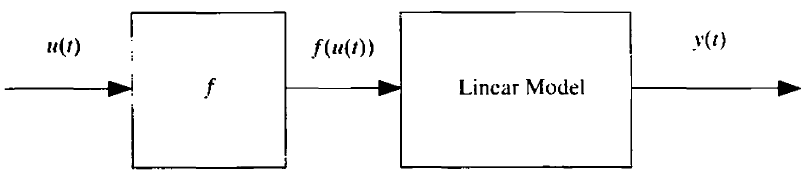
\includegraphics[width=\textwidth]{pictures/hammerstein}
\caption{Model Hammersteina \cite{21}.}
\label{hamm}

\vspace{0.5cm}

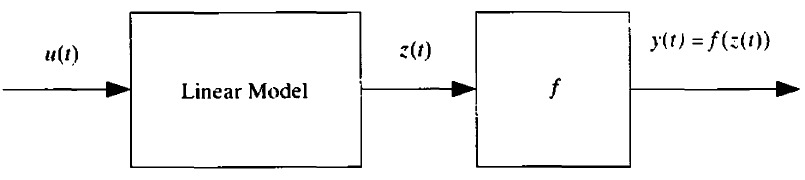
\includegraphics[width=\textwidth]{pictures/wiener}
\caption{Model Wienera \cite{21}.}
\label{wien}
\end{figure}

Modele te doskonale nadają się do identyfikacji systemów nieliniowych. Często w tym celu wykorzystywane są funkcje wielomianowe, sieci neuronowe czy systemy rozmyte \cite{150}.